\documentclass[12pt,a4paper,notitlepage]{article}
\usepackage[utf8]{inputenc}
\usepackage[english]{babel}
\usepackage{amsmath}
\usepackage{titling}
\usepackage{amsfonts}
\usepackage{amssymb}
\usepackage{pgfplots}
\usepackage{caption}
\usepackage{graphicx}
\usepackage{tikz-3dplot}
\usepackage{subcaption}
\usepackage{float}
\usepackage{adjustbox}
\usepackage{multirow,rotating}
\usepackage[autostyle]{csquotes}
\usepackage[toc,page]{appendix}
\DeclareUnicodeCharacter{20AC}{\euro}

\usepackage[backend=biber,style=authoryear-comp]{biblatex}
\addbibresource{Meine Bibliothek.bib}

\title{Market Definition of Platform Markets}
\date{\today}
\author{Ralf Dewenter, Ulrich Heimeshoff, Franziska Loew}

\begin{document}
\begin{titlepage}
	\maketitle
	\begin{abstract}
		Platform markets are characterized by the existence of indirect network effects that connect two or more market sides through a platform that internalizes these feedback effects. Conventional instruments of market definitions which consider price levels cannot easily applied in case of two-sided platform competition, as price structure of those markets are non-neutral. Instead of using prices, we use time series of quantities and simple correlation analysis to evaluate the substitutional relationship within two-sided media markets. As a benchmark model, we simulate a Cournot duopoly on order to calculate correlation coefficients for varying degrees of product differentiation and indirect network effects.
		
		\textbf{Keywords} two-sided markets, market definition, printed media, network effects

	\end{abstract}

\end{titlepage}

% JEL: D43, L40, L82
% ----------------------------------------------------------------------------------------------------
%  INTRODUCTION
% ----------------------------------------------------------------------------------------------------

\section{Introduction}

Market definition in two-sided markets is a complex and current challenge in antitrust analysis. While many recent cases, such as, e.g., EU ./. Google, Bundeskartellamt ./. Facebook and others deal with two-sided platform markets, no quantitative method has been developed yet which is applicable and suitable as a practical tool for market definition. As traditional methods developed for so called one-sided (or traditional) markets are no longer valid, new methods which account for the interelation of two-sided markets are typically too complex to be applied to actual cases. The interdependence of quantities and prices from both markets, caused by indirect network effects, leads to severe identification problems and therefore to demanding data requirements. For this reason, there is an emerging debate on whether or not two-sided markets should be defined at all and some authors recommend to completely abandon market definition, as it is considered useless and incoherent (Kaplow, 2010; Evans \& Noel,2005). However, competition authorities typically do not have the choice to completely abandon market definition. They are either obliged by law to properly define relevant markets or have at least to identify the closest competitors in order to evaluate possible effects of anti-competitive behaviour. Because of practical reasons, competition authorities therefore do typically not use quantitative methods but rather qualitative procedures to define two-sided markets.   

Two-sided or platform markets, are characterized by the existence of indirect network effects. Many two-sided buzsinesses are intermediaries or platforms that sell two different products to two different groups of agents. These two groups are interconnected by network effects as they mutually influence each other’s demand. The platforms recognize the interconnection and choose the price structure according to the relative size of the indirect network effects. In a more restrictive definition of two-sided markets, \cite{rochet_platform_2003} determine those markets as two-sided, if the price structure is non-neutral, i.e., the volume of transactions and the participation levels vary as the price structure varies, holding the price level constant. This definition stresses the importance of the distinction between the price level, which is the sum of the prices charged by a platform on both sides, and price structure, which is the allocation of the price level among the two sides. Traditional antitrust instruments like the SSNIP test are designed for single-sided markets, using the price level to analyze a market. Drawing from the economic literature on market definition with interdependencies in demand, it can be shown that these instruments cannot easily be applied in case of two-sided platform competition (\cite{noel_analyzing_2005} \cite{filistrucchi_market_2013}).

Although two-sided markets are not invented by the digital revolution, digital markets very often demonstrate a market structure with two or more consumer-groups that are related via indirect network effects and are connected by platforms. A very prominent example can be found within the search engine market, where Google connects at least two market-sides: the demand for search query and the demand for placing advertisement. It can easily be seen, that advertisers value a big group on the other market side, as their scope and therefore the effectiveness of advertisement grows. The value of the search query on the other market side might be influenced negatively or positively by the amount of advertisement. This indirect network effect pretty much depends on the quality of the advertisement and on the consumers demand on personalized advertisement.

Two-sided markets can also be found within more traditional markets like credit cards, newspapers or shopping malls. These markets play an important role when analyzing the nature of two-sided markets as they offer an explicit market structure and available data. Requirements that cannot easily be found within digital markets due to rapidly changing market dynamics. Nevertheless, the rapid growth of digital markets calls for an analytical tool that can be applied to define the relevant market.

Based on economic reasoning we will explain why the application of a SSNIP test - being the most important analytical tool for regulatory and antitrust cases in the EU - on a two-sided market leads to a erroneous market definition. Furthermore we present an approach to analyze market structure by looking at the cross correlations of quantities of potential competitors. As a benchmark for the cross correlation coefficients we will simulate a Cournot duopol model. 
% Dass wir den SSNIP test beschreiben stimmt ja nicht (mehr)

This paper aims at filling this gap of quantitative two-sided market definition. We developed a new method for the identification of competitors in two-sided markets by using time series methods and simple correlation analysis. At first, time series on quantities from both markets are adjusted by time series models in order to prevent spurious regressions. We use quantities instead of prices as (i) substitutability is directly reflected in quantities but not necessarily in prices (ii) indirect network effects are directly linked to quanitites  and (iii) two-sided markets such as platform markets typically characterized by zero prices on either of the sub markets. Next, either cross-correlation functions or simple contemporary correlations are calculated to identify the substitutability of different products. The procedure is applied to reader and advertising markets of different popular magazines genres. 

To evaluate the degree of substitutability between different media outlets, we first build a simple model of two-sided markets. We then use Monte Carlo simulations in order to calculate correlation coefficients for varying degrees of product differentiation as well as indirect network effects. A comparison of empirical correlations with Monte Carlo results can then be used to identify the degree of substitutability. 




The paper proceeds as follows: chapter \ref{litrev} presents a review of the relevant literature on market definition and two-sided markets and analyses the consequences of applying a SSNIP test for market definition on two-sided markets; chapter \ref{model} presents a Cournot duopol model of platform competition and the results of a Monte Carlo simulation for this model; chapter \ref{empirical}  explains how we use empirical data to test our approach of market definition using cross-correlation functions of quantities in media markets.  


% -----------------------------------------------------------------
% LITERATURE
% -----------------------------------------------------------------



\section{Literature review}\label{litrev}
This paper is related to a relatively recent line of economic literature, investigating the implications of two-sided markets on competition policy and offering different approaches to deal with the feedback effects between demand on multiple market sides. While the first policy contributions mainly criticized the application of standard policy to those markets (\cite{wright_one-sided_2004}; \cite{leonello_horizontal_2010}; \cite{chandra_mergers_2009}), more recent work has also intended to suggest alternative approaches (\cite{argentesi_estimating_2007}; \cite{song_estimating_2015}). We try to contribute to the latter by offering a new approach to define a two-sided market. 

The literature of two-sided markets was pioneered by the theoretical work of \cite{caillaud_chicken_2003}, \cite{rochet_platform_2003}, \cite{evans_antitrust_2003} and \cite{armstrong_competition_2006}, whereby the definition given by \cite{evans_antitrust_2003} can be seen as a particular case of the more general definition proposed by \cite{rochet_platform_2003} (\cite{filistrucchi_identifying_2012}). \cite{rochet_platform_2003} as well as \cite{armstrong_competition_2006} both provide a theoretical concept to analyze how platforms chose prices in a market with two consumer sides (networks) showing indirect network effects. However, there are a number of modeling differences between the two articles with regard to (a) the platform's cost structure, (b) the fee the consumers on both market sides have to pay and (c) the source of consumer heterogeneity. A more detailed discussion of these assumptions with regard to our approach is provided in Chapter \ref{model}.  

As mentioned above, earlier policy contributions criticize the application of standard competition policy on markets that exhibit at least one indirect network effect. \cite{evans_antitrust_2003}, \cite{evans_industrial_2007} \cite{wright_one-sided_2004} and \cite{kaiser_price_2006} are prominent examples of papers that have focused on competition policy on two-sided markets. They have pointed out, that in the presence of indirect network externalities the efficient price structure does not reflect the ratio of marginal cost, nor does increased competition necessarily leads to a more efficient market outcome or merger leads to increased prices.\footnote{\cite{malam_mergers_2011} uses an oligopoly model of competition with differentiated products (based on the approach of \cite{salop_monopolistic_1979}) where ad-sponsored media platforms charge a zero price to viewers when competing simultaneously for advertisers. He shows, that mergers among ad-sponsored platforms have a competition-intensifying effect, which offsets the incentive to increase prices on the advertiser side.} They show that relying on conventional methods to analyze mergers in two-sided markets will lead to significantly different results than using methods that explicitly incorporate the two-sided nature of those markets. \cite{evans_antitrust_2003} argues that defining a relevant market for antitrust purposes looking at only one side can lead to a market definition which is too narrow. In a more recent study \cite{evans_analysis_2008} analyze the Google and DoubleClick case, confirming, that the Lerner pricing formula does not hold for two-sided markets. While predatory pricing is a practice that harms competition in case of traditional industries\footnote{Industries with only one market side.}, selling a product below marginal cost\footnote{Or even for free, as is the case for the search-engine market as well as many digital markets.} can be a profit maximizing strategy rather than an attempt to predate in a two-sided market (\cite{wright_one-sided_2004}). \cite{wright_one-sided_2004} also argues, that increased competition does not necessarily lead to more efficient prices from the social point of view. An analysis of the Canadian newspaper industry shows, that mergers in two-sided markets may not necessarily lead to higher prices for either side of the market. Even a merger to monopoly might raise welfare and do so even in the absence of efficiency gains (\cite{leonello_horizontal_2010}). These papers emphasizes the need for alternative approaches to adopt competition policy that adequately hits the requirements of two-sided markets. 

The actual handling of antitrust issues regarding two-sided markets often lack the identification of indirect network effects. Even if indirect network effects are detected, the definition of the relevant market still remains a challenging task. This is mainly attributable to the fact that available analytical tools of market definition are not applicable for markets with interconnected demands as they consider price levels instead of price structure. The analysis of substitutional relationships is a well-established practice to define the relevant market. The European Commission uses the hypothetical monopolist test (the SSNIP test) which identifies the smallest relevant market through demand-substitutability of a certain product. If a small but significant, non-transitory price increase (5\% - 10\%) is profitable for the hypothetical monopolist then there is a relevant market (\cite{motta_competition_2004}). 

Using this analytical tools to define markets for a product offered on one side of a two-sided market can result in significantly overstating or understating the breadth of the market (\cite{evans_analysis_2008}). Due to the fact that platforms need to balance the preferences of two (or more) different groups of consumers, they often behave in a way that would not be efficient for traditional firms (e.g. they set prices $<$ marginal cost) (\cite{chandra_mergers_2009}).

\cite{evans_market_2012} uses the following example to illustrate the problem of the SSNIP test in platform markets. Suppose a small but significant, non-transitory price increase is profitable on one side under the assumption that nothing changes on the other market side of the platform included in the hypothetical monopoly. Therefore one could conclude that the products considered constitute a relevant antitrust market. However, a price increase on one side results in a reduction of demand by customers for that side and, through positive feedback effects, a reduction in the demand for the other side; the decline in demand on the other side further reduces the demand on the first side. Consequently, one might conclude after considering the positive feedback effects that the price increase is unprofitable. In that case the market is defined too narrowly .

The existence of positive feedback effects between demands of the two market sides calls for an optimal strategic behavior that varies widely from profit maximization on conventional one-sided markets. The SSNIP test might be applied in a modified way as shown by \cite{filistrucchi_market_2013} as well as \cite{evans_defining_2007}, who include the profit change in consideration of demand elasticity and indirect network effects. \cite{white_insulated_2012} present a UPP formulae for two-sided markets assuming that firms charge insulating tariffs, meaning that platforms choose quantities and then support those quantities by the corresponding insulating tariffs and \cite{noel_analyzing_2005} suggests an extension of the Critical Loss Analysis as an alternative method to define two-sided markets.\footnote{See \cite{evans_two-sided_2012} and \cite{filistrucchi_identifying_2012} for a discussion of market definition in two-sided markets.} Although these models are correct in theory, they show various problems when implemented in practice. 

\cite{filistrucchi_ssnip_2008} suggest a distinction of the two-sided markets regarding the observability of transaction costs.\footnote{Whereas \cite{filistrucchi_ssnip_2008} uses the terms “media type” and “payment card type”, \cite{filistrucchi_market_2013} use the terms “non-transaction” and “transaction” marktes.} In the "payment card type" market the platform can observe the transaction cost between the two market sides, whereas in the "media type" market the transaction cost does not exist (or is not observable to the platform, e.g. reader reads an ad). In \cite{filistrucchi_market_2013} the authors point out, that in two-sided non transaction markets, two (interrelated) markets need to be defined, while in transaction markets, only one market side should be defined. \cite{emch_market_2006} and \cite{alexandrov_antitrust_2011} show how a SSNIP test should be performed in a two-sided non transaction market. However, as transaction markets might exhibit asymmetric relationships in exceptional cases, this distinction cannot easily be applied. 

One well-known problem of most of those analytical tools is the procurement of necessary information. Due to the complexity of the two-sided market, this task is particularly difficult, as the scope of the indirect network effects has to be known for this analysis. A SSNIP test requires both qualitative data on substitutional behavior of consumers and quantitative market data. The data collection always is challenging, costly and time expensive and this is all the more true in case of two-sided markets as data has to be collected for two market sides. Even though the data required is available, two-sided markets poses special analytical challenges not allowing reliable conclusions about the market size. 

A determining factor are the platforms' pricing strategies. As mentioned above, price strategies have to be distinguished between the price level - the sum of the prices on both market sides - and price structure - the allocation of the price level among the two sides depending on the indirect network effects (\cite{rochet_two-sided_2006}). In an extreme case, prices on one market side can not be observed, as one market side benefits from a strong positive indirect network effect, affecting the other market side. In this case, the consumer group that receives the strong positive indirect network effect has to pay for the value gain. One market side therefore subsidizes the other depending on the relation of network effects. One can argue, that one market side does not pay a monetary price, but consumers pay with their attention or their data. The absence of monetary prices is not a rare phenomenon in digital markets. In the prominent example of the search engine market, the search market is subsidized by the advertiser market, because the extra value the advertiser side gets from an additional searcher is much higher, than the indirect network effect from the advertiser to the searcher\footnote{Which also can be assumed to be negative.}. Without monetary prices it will be impossible to analyze a hypothetical percentage price increase. To assign a value to the hedonic price, a quality benchmark is needed which itself is a difficult task (\cite{filistrucchi_market_2013}). Furthermore the consideration of prices does not capture the dynamic nature of a two-sided market, where firms rather use innovation and quality as strategic parameters (\cite{evans_economic_2002}; \cite{gual_market_2003}). 

The presence of relatively high fix cost and low marginal cost is another reason why the evaluation of prices does not represent an adequate measure, especially for online markets. In case of declining average cost due to fixed cost degression, the conventional SSNIP-test would define the relevant market to narrowly (\cite{gual_market_2003}). The same is true for endogenous sunk cost. In both cases  the relevant strategic parameters are others than the prices.

Beside the problems that arise when the SSNIP test is applied for two-sided markets, there are several general difficulties with this tool. The so called Cellophane-Fallacy  presents one well-known problem of the SSNIP-test (\cite{schaerr_cellophane_1985}). If the observed market price already exceeds the competitive price level, substitutional relationships between products are overestimated and market definition will be too broad. This problem is even more true for two-sided markets where a price on one market side seems to be “too low” (price is lower than monopoly price without feedback effects) while it is “too high” on the other market side (price is higher than monopoly price) (\cite{dewenter_einfuehrung_2014}).

A modified SSNIP test has to take into account all of these particular challenges when defining a two-sided market. Additional to this demanding task, the dynamic development of digital platform markets requires a fast and effective tool. The problems described make it evident that the SSNIP test – even in a modified way – is not an adequate tool when it comes to the task to define a relevant market that shows indirect network effects between two market sides, especially in the case of digital markets. This also applies for other analytical tools that analyze cross-price-elasticities. The reason is that market prices in two-sided markets cannot be interpreted in the conventional way as they reflect the relation of indirect network effects between the market sides. However, quantity measures offer an alternative approach to analyze substitutability of relevant goods. 

This paper contributes to the body of research that provides practical suggestions to practitioners. We use data on quantity to analyze substitutional effects on two-sided markets. The advantage of using quantity data is clear: As price levels and price structure in two sided markets are closely linked to the scope of indirect network effects, they can hardly be analyzed in the conventional way of antitrust economics. 




% ------------------------------------------------------------------------------
% MODEL
% ------------------------------------------------------------------------------





\section{A model of two-sided markets}\label{model}
In order to observe quantities from two-sided markets, we first develop a model of duopolistic platforms offering differentiated products (or services) to two different groups of users. Both sides of the market are assumed to be interrelated by indirect network effects and platforms to set quantities simultaneously. Consider therefore an industry with a continuum of potential users on each side $k = a,b$ of the market, with mass normalized to unity, and two platforms, $i = 1,2$, which enable the two groups to interact. Following \cite{shubik_market_1980} we introduce a quadratic utility function for each side of the market as\footnote{See also \cite{dixit_model_1979} and \cite{kind_competition_2006}}

\begin{equation}\label{4.1}
u_i^a = \nu^a q_i + \nu^a q_j-\frac{\beta^a q^2_i+ \beta^a q^2_j+ 2 \theta q_i q_j}{2}-(p_i-d s_i)q_i
\end{equation} and 

\begin{equation}\label{4.2}
u_i^b = \nu^b s_i + \nu^b s_j -\frac{\beta^b s^2_i+ \beta^b s^2_j+2 \mu s_i s_j}{2}-(r_i-g q_i)s_i.
\end{equation}

For $i=1,2, i \neq j$, we assume (i) $\nu^k > 0$, (ii) $\beta^k > 0$, (iii) $\beta^k>\vert\theta,\mu\vert$, where $\nu^k$ is a fixed benefit the agent obtains if she uses platform $i$ on market side $a$ or $b$ respectively.\footnote{\cite{weyl_price_2010} refers to it as the membership benefit or cost.} Parameter $\theta \in (0,1)$ and $\mu \in (0,1)$ indicate the degree of substitutability of both products, with $\theta (\mu) = 1$ indicating perfect substitutes and $\theta (\mu) = 0$ indicating monopolistic markets. $q_i$ and $s_i$ measure consumption of both product on platform $i$. By normalizing  population to one, we can interpret $q_i$ ($s_i$) as each individual’s consumption of product $i$ on market side $a$ ($b$), or as the network size of the platform $i$ on the respective market side.

The standard quadratic utility functions are also expanded by the cost-terms $(p_i-d s_i)q_i$ and $(r_i-g q_i)s_i$, respectively (\cite{kind_business_2009}). User's utility therefore depends on respective prices ($p_i$ and $r_i$) as well as on the network size of the opposite market side ($d$ and $g$). Hence, $d$ and $g$ describe the magnitude and the direction of the two indirect network effects. 

Solving for the FOCs of the consumer problem, given by $\frac{\delta u_i^a(q_i,q_j,s_i,p_i)}{\delta q_i}=0$ and  $\frac{\delta u_i^b(s_i,s_j,q_i,r_i)}{\delta s_i}=0$ utility can be expressed as

\begin{equation}\label{utility_a}
u_i^a = \nu^a-\beta^a q_i - \theta q_j +ds_i - p_i
\end{equation}
and
\begin{equation}\label{utility_b}
u_i^b=\nu^b-\beta^b s_i - \mu s_j +gq_i - r_i.
\end{equation} 

User heterogeneity on each side of the market can be modeled in two dimensions: the value of membership and the value of indirect network effects.\footnote{\cite{weyl_price_2010}, \cite{rochet_platform_2003} and \cite{armstrong_competition_2006} refer to this as the interaction value or the per-transaction value.} \cite{rochet_platform_2003} assume $v^k=0$ and that users have heterogeneous interaction values. Put differently, \cite{rochet_platform_2003} assume that the strength of indirect network effects vary with agents and platforms. \cite{armstrong_competition_2006}, in contrast, assumes that the indirect network effects $d,g$ only depend on the market side and allows for heterogeneous membership values.\footnote{\cite{rochet_platform_2003} as well as \cite{weyl_price_2010} allow agents to be heterogeneous along the two dimensions for the monopoly case.} We follow \cite{armstrong_competition_2006} in assuming that the scope of the indirect network effect depends on the market side, but not on agents or platforms. Our formulation of utility also coincides with \cite{armstrong_competition_2006} in that we assume lump-sum fees rather than per-transaction fees. 

Equations \ref{utility_a} and \ref{utility_b} can then be converted to obtain the inverse demand functions

\begin{equation}
p_i=\nu^a-\beta^a q_i - \theta q_j +ds_i
\end{equation}
and
\begin{equation}
r_i=\nu^b-\beta^b s_i - \mu s_j +gq_i.
\end{equation} 

This system of inverse demands illustrates the importance of assumption (iii): The closer $\theta, \mu$ to $\beta^k$, the closer substitutes are the two products, with $\theta, \mu \to \beta^ k$ as the limiting case. Equations \ref{4.1} and \ref{4.2} imply, that consumers utility from the indirect network effect is higher the more she uses the platform (\cite{kind_business_2009}). Keeping everything else equal, demand on market side $b$ has a positive impact on demand on market side $a$ if the indirect network parameter has a positive sign ($d > 0$). Same is true for market side $b$ and the parameter $g$. While most two-sided markets are characterized by two positive indirect network effects, especially ad-supported platforms such as media platforms are likely to show a positive as well as a negative effect. Demand for advertising increases with the size of media platform's audience. At the same time, when advertising is a nuisance to the audience, a higher amount of advertising would result in a lower demand for content.

Following \cite{armstrong_competition_2006}, we assume that the cost of platform $i$ is market-side specific and that they are incurred when an user joins the platform, so that platform's $i$ total cost is $c_i q_i+f_i s_i$ for some per-user cost $c_i$ for serving group $a$ and per-user cost $f_i$ for serving group $b$. The profit of platform $i$ therefore can be expressed as 

\begin{equation}\label{eq:profit}
\pi_i=(p_i-c_i)q_i+(r_i-f_i)s_i.
\end{equation}

Both platforms set $q_i$ and $s_i$ to maximize profits, given the choices of its rival. Substituting unique demands into \ref{eq:profit} for $i=1,2$, and using first order conditions, optimal quantities, prices and profits can be derived \footnote{See Appendix \ref{appendix_model} for optimal quantities}. Subsequently, optimal quantities can be used for simulating times series and correlation coefficients. 


 As optimal quantities are far from being easy to interpret, we present a simpler version of $q_i, s_i$ assuming $\nu^k, \beta^k=1$  as well as $c_i=f_i=0$. Equilibrium quantities are then

\begin{equation}\label{eq_quantities1}
	q_i=\frac{2+d+g+\mu}{4-(d+g)^2+\mu\theta+2(\mu+\theta)}
\end{equation}

and

\begin{equation}\label{eq_quantities2}
	s_i=\frac{2+d+g+\theta}{4-(d+g)^2+\mu\theta+2(\mu+\theta)}.
\end{equation}

As long as indirect network effects are positive, both quantities increase with $d$ and $g$. It can also be shown that $\frac{\partial q_i}{\partial \mu}<0$, $\frac{\partial q_i}{\partial (d+g)}>0$, $\frac{\partial s_i}{\partial \theta}<0$, $\frac{\partial s_i}{\partial (d+g)}>0$ as long as $0<(d+g)<2$. As positive indirect network effects have a positive impact on willingness to pay, quantities are also increasing with higher network effects. A higher degree of substitutability increases competition and reduces quantities.  






% ------------------------------------------------------------------------------
% MONTE CARLO
% ------------------------------------------------------------------------------




\section{Monte Carlo simulation}

We are interested in the market behavior of platforms depending on a change in parameters $d, g$ and $\theta, \mu$. More precisely our aim is to analyze the correlation coefficient of quantities depending on the degree of substitution and the indirect network effects. For this purpose, we use Monte Carlo simulation to obtain benchmark correlation coefficients, by simulating external shocks in platforms' marginal costs. 

We assume marginal costs to consist of two parts: (1) A market-specific term, which is common for both platforms and (2) an individual firm-specific cost-shock, assumed to occur in every period such that marginal costs follow a random walk (\cite[241]{harrington_detecting_2008}, \cite{paha_empirical_2011}). Assumption (1) is rational if we assume homogeneous input-factors are purchased from a perfectly competitive market. This assumption is relaxed by the platform-specific cost-shock which arises asymmetry between the platforms. This asymmetry might be due to individual negotiations between a platform and its service-provider. Moreover, asymmetry can be assumed to be larger, the smaller $\theta$ and $\mu$ as a high degree of heterogeneity might cause more asymmetric input costs, while homogeneous products should be produced with more symmetric input costs. 



A cost function of platform $i$ for $n$ simulated markets with the corresponding characteristics can then be described as
\begin{equation}
f_{i,n} = a^a_n+a^a_{i,n},
\end{equation} and 
\begin{equation}
c_{i,n} = a^b_n+a^b_{i,n},
\end{equation}
with $a_{k,t} \in [0.001;0.0001]$ for the common cost shock and $a_{ki,t} \in [0.01;0.001] $ for the platform-specific cost shock. Cost-asymmetry among firms is therefore modeled by adding a firm-specific term $a_{ki,t}$ to the market-specific marginal cost. 

We randomly generate a dataset of $n=1000$ two-sided markets, by randomly generating $n=1000$ values for $f_i$ and $c_i$, respectively.\footnote{More precisely, we generate $n$ values for $a^a_n$ and $a^a_{i,n}$ and $a^b_n$ $a^b_{i,n}$ respectively.} Using the simulated values for $f_i$ and $c_i$ we are able to calculate the equilibrium quantities for every market on both market sides. As we are interested in substitutional relationship between the equilibrium quantities to define the market, we then calculate correlation coefficients from quantities. According to a Cournot duopoly we expect $q_i$ and $q_j$, as well as $s_i$ and $s_j$ to be correlated negatively. 

Table \ref{tab_ccf_simulated} includes correlation coefficients between $q_1$ and $q_2$ for different degrees of substitutability and varying sums of network effects. With maximum product differentiation $\theta=0$ correlation coefficients are insignificantly different from zero, however, with increasing substitutability correlation coefficients increase. Moreover, stronger network effects lead to higher correlations. In case that network effects are neglectable, correlation is moderate ($\rho=-0.501$) for moderate product differentiation ($\theta=0.5$) and relatively high ($\rho=0.792$) for low perfect substitutes ($\theta=1$). With increasing network effects, interdependency of the markest becomes stronger and therefore correlation between quantities from identical markets goes up. 

Figure \ref{fig_QQ} illustrates the relation between the sum of the indirect network effects $d+g$ and the correlation of quantities $\rho(q_i,q_j)$ on market side $a$, depending on the substitution parameter $\theta$ \footnote{For simplicity we assume $\mu=\theta$}. Keeping ($d+g$) constant, a high degree of homogeneity causes negative correlations to increase, which is consistent with what we would observe in markets without indirect network effects. Homogeneous products ($\mu=1$) cause a high degree of competition, which leads to high negative correlation of quantities, whereas a small degree of homogeneity $\theta \to 0$ results in little or no substitutional effects. Keeping instead the correlation coefficient constant, an increasing total sum of indirect network effects suggests less competition. The higher the absolute amount of ($d+g$), the higher the negative correlation between the quantities keeping $\theta$ constant. As we assume network effects to be equal for both platforms, a higher interdependency of the markets will result in a higher correlation of quantities. 

Both, indirect network effects and parameters of product differentiation are unknown in our model. Therefore, in order to get a relative exact impression of substitutability, the strength of indirect network effects have to determined in advance. This can be achieved by either making theoretical assumptions about indirect network effects or by estimating these effects empirically. Most of the literature related to the quantification of the indirect network effects have based their analysis on electronic payments system industries (\cite{ackerberg_quantifying_2006}; \cite{rysman_empirical_2007}) or magazine and newspaper industries (\cite{kaiser_price_2006}, \cite{argentesi_estimating_2007}). Even though such an investigation on the INE gives empirical evidence, the drawback is twofold: First, many antitrust cases cannot meet the huge data requirements for an empirical investigation. Second, theoretical assumption have to be made that might not reflect the industry characteristics adequately. 

To overcome problems connected with data requirements and empirical modeling, we restrict our analysis to the assumptions of our theoretical model. By simulating quantities as a function of indirect network effects as well as differentiation parameters, we are able to estimate a range of substitutability depending on different strengths of the indirect network effects. Assuming a specific range of network effects and estimating correlation coefficients can then be used to limit the most likely range of substitutability.  



%\begin{figure}[H]
%	\centering
%	\caption{Simulated Correlation of $q_i$ and $q_j$}
%	\begin{adjustbox}{width=\textwidth}	
%	\input{QQ.tex}
%	\label{fig_QQ}
%\end{adjustbox}
%\end{figure}


\begin{table}[ht] \centering 
\caption{Simulated Correlation Coefficients of $q_1$ and $q_2$}
\label{tab_ccf_simulated}
\begin{adjustbox}{width=\textwidth}	
\small
\begin{tabular}{@{\extracolsep{5pt}} cccccccccccc} 
\\[-1.8ex]\hline 
\hline \\[-1.8ex] 
$d+g$ & $\theta=0$ & $\theta=.1$ & $\theta=.2$ & $\theta=.3$ & $\theta=.4$ & $\theta=.5$ & $\theta=.6$ & $\theta=.7$ & $\theta=.8$ & $\theta=.9$ & $\theta=1$\\ 
\hline \\[-1.8ex] 
-.9 & $0.010$ & $$-$0.178$ & $$-$0.321$ & $$-$0.477$ & $$-$0.616$ & $$-$0.722$ & $$-$0.824$ & $$-$0.885$ & $$-$0.941$ & $$-$0.974$ & $$-$0.994$ \\ 
-.8 & $0.025$ & $$-$0.152$ & $$-$0.264$ & $$-$0.423$ & $$-$0.558$ & $$-$0.644$ & $$-$0.775$ & $$-$0.839$ & $$-$0.907$ & $$-$0.946$ & $$-$0.979$ \\ 
-.7 & $$-$0.002$ & $$-$0.130$ & $$-$0.313$ & $$-$0.374$ & $$-$0.499$ & $$-$0.622$ & $$-$0.691$ & $$-$0.794$ & $$-$0.858$ & $$-$0.917$ & $$-$0.953$ \\ 
-.6 & $0.007$ & $$-$0.086$ & $$-$0.265$ & $$-$0.430$ & $$-$0.488$ & $$-$0.574$ & $$-$0.650$ & $$-$0.751$ & $$-$0.837$ & $$-$0.891$ & $$-$0.921$ \\ 
-.5 & $$-$0.019$ & $$-$0.098$ & $$-$0.197$ & $$-$0.289$ & $$-$0.437$ & $$-$0.572$ & $$-$0.605$ & $$-$0.712$ & $$-$0.786$ & $$-$0.855$ & $$-$0.897$ \\ 
-.4 & $$-$0.003$ & $$-$0.067$ & $$-$0.226$ & $$-$0.264$ & $$-$0.395$ & $$-$0.507$ & $$-$0.582$ & $$-$0.692$ & $$-$0.758$ & $$-$0.822$ & $$-$0.865$ \\ 
-.3 & $0.049$ & $$-$0.100$ & $$-$0.156$ & $$-$0.264$ & $$-$0.414$ & $$-$0.519$ & $$-$0.553$ & $$-$0.643$ & $$-$0.694$ & $$-$0.790$ & $$-$0.831$ \\ 
-.2 & $$-$0.021$ & $$-$0.117$ & $$-$0.207$ & $$-$0.324$ & $$-$0.345$ & $$-$0.462$ & $$-$0.576$ & $$-$0.627$ & $$-$0.691$ & $$-$0.767$ & $$-$0.816$ \\ 
-.1 & $0.035$ & $$-$0.095$ & $$-$0.192$ & $$-$0.321$ & $$-$0.363$ & $$-$0.420$ & $$-$0.569$ & $$-$0.626$ & $$-$0.713$ & $$-$0.745$ & $$-$0.800$ \\ 
0 & $0.014$ & $$-$0.099$ & $$-$0.221$ & $$-$0.312$ & $$-$0.444$ & $$-$0.501$ & $$-$0.556$ & $$-$0.595$ & $$-$0.669$ & $$-$0.774$ & $$-$0.792$ \\ 
.1 & $0.007$ & $$-$0.134$ & $$-$0.213$ & $$-$0.314$ & $$-$0.386$ & $$-$0.472$ & $$-$0.526$ & $$-$0.634$ & $$-$0.708$ & $$-$0.748$ & $$-$0.793$ \\ 
.2 & $0.031$ & $$-$0.093$ & $$-$0.194$ & $$-$0.253$ & $$-$0.419$ & $$-$0.521$ & $$-$0.555$ & $$-$0.666$ & $$-$0.693$ & $$-$0.796$ & $$-$0.818$ \\ 
.3 & $0.057$ & $$-$0.113$ & $$-$0.244$ & $$-$0.316$ & $$-$0.387$ & $$-$0.440$ & $$-$0.595$ & $$-$0.637$ & $$-$0.746$ & $$-$0.800$ & $$-$0.838$ \\ 
.4 & $0.070$ & $$-$0.111$ & $$-$0.197$ & $$-$0.312$ & $$-$0.407$ & $$-$0.541$ & $$-$0.592$ & $$-$0.673$ & $$-$0.759$ & $$-$0.823$ & $$-$0.859$ \\ 
.5 & $0.017$ & $$-$0.176$ & $$-$0.219$ & $$-$0.287$ & $$-$0.452$ & $$-$0.499$ & $$-$0.661$ & $$-$0.736$ & $$-$0.779$ & $$-$0.835$ & $$-$0.901$ \\ 
.6 & $0.010$ & $$-$0.070$ & $$-$0.266$ & $$-$0.384$ & $$-$0.496$ & $$-$0.580$ & $$-$0.641$ & $$-$0.753$ & $$-$0.824$ & $$-$0.885$ & $$-$0.923$ \\ 
.7 & $0.006$ & $$-$0.092$ & $$-$0.241$ & $$-$0.356$ & $$-$0.536$ & $$-$0.622$ & $$-$0.728$ & $$-$0.795$ & $$-$0.870$ & $$-$0.923$ & $$-$0.956$ \\ 
.8 & $$-$0.006$ & $$-$0.111$ & $$-$0.262$ & $$-$0.455$ & $$-$0.543$ & $$-$0.667$ & $$-$0.752$ & $$-$0.840$ & $$-$0.900$ & $$-$0.959$ & $$-$0.980$ \\ 
.9 & $0.008$ & $$-$0.143$ & $$-$0.304$ & $$-$0.463$ & $$-$0.612$ & $$-$0.731$ & $$-$0.815$ & $$-$0.891$ & $$-$0.935$ & $$-$0.976$ & $$-$0.994$ \\
\hline \\[-1.8ex] 
\end{tabular} 
\end{adjustbox}
\label{tab:ccf_sim}
\end{table} 


% ----------------------------------------------------------------------------------------------------
%  EMPIRICAL ANALYSIS
% ----------------------------------------------------------------------------------------------------




\section{Empirical analysis}\label{empirical}

\subsection{A Simple method for detecting substitutional relationships in two-sided markets}

This section presents a simple method for detecting substitutional relationships in two-sided markets using cross-correlation functions as well as simple contemporary correlations. To test our approach of identifying substitutional relationships we use data on German popular magazines which are a typical example of two-sided markets. Magazine publishers serve a reader market as well as an advertising market, which are both interrelated by indirect network effects. Furthermore, data on German popular magazines is available for a broad range of differentiates products, for both, reader advertising markets. We are therefore able to identify possible substitutional products from a relatively high number of genres. Identification of possible substitutes has to be based on plausibility considerations. As popular magazines are typically highly differentiated, characteristics such as price level, layout, frequency of publication, but also socio-demographic factors of readers can help to identify possible competitors.  

As data form identical markets are typically affected by the same external influences, time series of prices and quantities are usually overlapped by common patterns. While quantities are strategic substitutes we expect to find negative contemporary correlations between substitutes. However, quantities as well as prices set by platforms from the same market or industry typically show identical patterns such as, e.g, seasonality, common trends or cyclical behavior. In order to prevent spurious regressions identical patterns have to be removed before an analysis of substitutability can be applied. For this purpose, we first apply different prewithening procedures. To prewhiten the quantities from both market sides we use different methods. At first, we apply a methods proposed by \cite{dewenter_essays_2004}. All series from similar markets which show the same patterns are regressed on each other including a trend and a constant. Next, different time series models such as ARMA and ARIMA models are applied for prewhitening matters (see \cite{box_time_2008}). The results form different models are used for a comparison.

Next, we are able to calculate either simple correlation coefficients or cross correlation functions and to compare the results with simulated correlations. Using cross correlation functions instead of simple correlation coefficients allows us to analyze not only contemporary correlation but also possible effects such as shifts in quantities from one magazine to an other. These shifts typically occur with market entry of new products. Given that all competitors compete for a longer period, contemporary correlation coefficients should be an adequate measure. 



\section{Data}\label{sec:data}

Data used in this study is extracted from the online magazine database ``PZ Online'' (Public Magazines Online) which provides (inter alia) information on circulation, advertising volumes and prices for al high number of magazines form different genres.\footnote{PZ Online is provided by the German association of magazine publishers (Verband Deutscher Zeitschriftenverleger) to provide advertising customers with necessary information on possible advertising platforms.} In order to address rather different genres and markets we use data on news magazines as well as on women's and TV magazines. 

To account for quantities in reader and advertising markets we use circulation numbers and advertising pages per copy, respectively. 
Even though the dataset contains data from 2003 to date we restrict our analysis to different two and three-year intervals (see Table \ref{tab:sample selection} for an overview of our samples). The reasoning behind subsampling is two-fold: First, as data availability often plays a crucial role for any economic policy analysis, using shorter periods allows us to prove that our approach is suitable even with low data availability. 
Second, antitrust concerns are often related to certain periods as markets develop constantly. Additionally, during recent years, print media have been subject to decreasing circulation and declining advertising revenues due to digitalization \footnote{For more information see \cite{cabyova_impact_2014} or \cite{picard_digitization_2011}}. Using data on magazine products proves that also markets with either decreasing or increasing market volumes can be subject of our approach.

\begin{center}
\begin{table}[htbp]
	
	\caption{Subsamples}
\begin{adjustbox}{width=\textwidth}	
\begin{scriptsize}
\bigskip\begin{tabular}{llllllll}
\hline 
	 Segment 	& Titles & & & Period &  & Frequency & Obs \\ \hline
	 &  &  &  & Begin & End &  &  \\ \hline
	News magazines 		& FOCUS & Der Spiegel & Stern & 2004 / 33 & 2006 / 33 & weekly & 105 \\ \hline
	 &  &  &  & 2013 / 33 & 2015 / 33 & weekly & 105 \\ \hline
	TV magazines 			& TV Movie & TV Spielfilm & TV Digital & 2012 / 15 & 2015 /15 & biweekly & 79 \\ \hline
	Women's magazines	& Brigitte & Freundin & Für Sie & 2012 / 15 & 2015 /15 & biweekly & 79 \\ \hline
\end{tabular}
\end{scriptsize}
	\label{tab:sample selection}
\end{adjustbox}
\end{table}
\end{center}

\subsection{News Magazines} 

First published in 1947 ``Der Spiegel'' had a monopoly on investigative journalism for a long time when Burda-Verlag entered the market in 1993 with a news magazine, FOCUS, claiming itself to be a close substitute to Der Spiegel. The latter instead opposed that FOCUS is an illustrative magazine similar to Stern, a magazine first published in 1946 by Gruner + Jahr \cite{kaltenhaeuser_abstimmung_2005}. In fact all three magazines differ regarding their editorial concept. Der Spiegel mainly focuses on complex political and social issues, whereas FOCUS also covers more non-political topics such as health and fitness. Stern has been a simple illustrative magazine without any political appeal until the 60s. It then started to address current political topics (\cite{vogel_populaere_1998}). Even though all three magazines have different editorial concepts, readership of Der Spiegel, FOCUS and Stern does not differ significantly regarding their socio-demographic characteristics, but their political orientation: While FOCUS is rather a conservative outlet, the coverage of Der Spiegel can be considered as left-wing. Stern which reporting is less political, can be located somewhere in between (\cite{kaltenhaeuser_abstimmung_2005}). Having this in mind, we do not expect strong competition in the reader market between the magazines as, e.g., a "left-wing" reader of Der Spiegel would probably not consider FOCUS as an adequate substitute et vice versa.\footnote{However as some of the readers might not have strong political preferences, we expect some kind of contemporary negative correlation, as final purchasing decisions will be influenced by cover stories and content. This assumption is supported by the fact that subscription is just a minor part of total sales (about 2-3 $\%$). We assume, if any, weak negative indirect network effects from the advertising market as the share of advertising pages per copy ranges between 2$\%$ and 8$\%$.} All three magazines offer several digital services (website and mobile apps) with mostly free content. 

Advertising demand on the other side is assumed to be strongly affected by the size and the characteristics of the readership of a certain magazine. However, in contrast to the reader market, political orientation should not matter as much as socio-demographic characteristics. We therefore expect the the degree of substitutability to be higher in the advertising market. All of the magazines might therefore be competitors in the advertising market.  

Graphical inspection of quantities (see figure \ref{fig_circ_fss1}) as well summary statistics (see table \ref{tab_news1}) shows, that in the reader market Stern and Der Spiegel have similar sales, whereas circulation of FOCUS is considerably smaller in both time samples. The overall mean decreased between the two periods by approximately 46$\%$, but sales of Der Spiegel are highest in both samples. Prices per copy remained the same without any fluctuations, with Der Spiegel being more expensive ($4.6 EUR$) than FOCUS and Stern who charge the same price per copy ($3.9 EUR$). On the advertising market, quantities of all three magazines are quite similar and show seasonal fluctuations (see figure \ref{fig_circ_fss1}). Summary statistics (\ref{tab_news2}) reveals, that advertising pages of Der Spiegel are lowest in terms of absolute and total values for both samples. Nevertheless, standard deviation is rather high, indicating high degree of fluctuation. Again, average quantities diminished between the time samples. This is true both for absolute and relative values. Looking at the prices per advertising side in the later sample shows, that prices for Der Spiegel is highest, followed by Stern and FOCUS. \footnote{There is no public available data on advertising prices before 2009. However, available data shows an increase of advertising prices from 2009 to 2016.}

\begin{figure}[H]
\caption{Reader Market}
\begin{minipage}
	\centering
	\input{../figs/circ_fss1.tex}
\end{minipage}
\hfil
\begin{minipage}
	\centering
	\input{../figs/circ_fss2.tex}
\end{minipage}
\label{fig_circ_fss1}
\end{figure}

\begin{figure}[H]
\caption{Advertising Market}
\begin{minipage}
	\centering
	\input{../figs/ads_fss1.tex}
\end{minipage}
\hfil
\begin{minipage}
	\centering
	\input{../figs/ads_fss2.tex}
\end{minipage}
\label{fig_ads_fss1}
\end{figure}

\begin{table}[!htbp] \centering 
  \caption{Summary Statistics: news magazines, reader market} 
	\label{tab_news1}
\begin{tabular}{@{\extracolsep{5pt}}lccccc} 
\\[-1.8ex]\hline 
\hline \\[-1.8ex] 
Statistic & \multicolumn{1}{c}{N} & \multicolumn{1}{c}{Mean} & \multicolumn{1}{c}{St. Dev.} & \multicolumn{1}{c}{Min} & \multicolumn{1}{c}{Max} \\ 
\\[-1.8ex]\hline 
\hline \\[-1.8ex] 
sales &&& 2004-2006 \\
\hline \\[-1.8ex]  
FOCUS & 105 & 170,252 & 34,250 & 111,395 & 275,025 \\ 
Der Spiegel & 105 & 442,254 & 49,155 & 334,815 & 548,854 \\ 
Stern & 105 & 395,620 & 41,844 & 306,323 & 499,818 \\  
\hline \\[-1.8ex] 
price per copy \\
\hline \\[-1.8ex] 
FOCUS & 105 & 4 & 0 & 4 & 4 \\ 
Der Spiegel & 105 & 5 & 0 & 5 & 5 \\ 
Stern & 105 & 4 & 0 & 4 & 4 \\
\\[-1.8ex]\hline 
\hline \\[-1.8ex] 
sales &&& 2013-2015 \\
\hline \\[-1.8ex] 
FOCUS & 103 & 78,641 & 20,301 & 48,179 & 184,981 \\ 
Der Spiegel & 105 & 249,184 & 23,247 & 203,587 & 320,651 \\ 
Stern & 105 & 215,036 & 18,908 & 174,604 & 272,927 \\ 
\hline \\[-1.8ex] 
price per copy \\
\hline \\[-1.8ex] 
FOCUS & 103 & 4 & 0 & 4 & 4 \\ 
Der Spiegel & 105 & 5 & 0 & 5 & 5 \\ 
Stern & 105 & 4 & 0 & 4 & 4 \\ 
\hline \\[-1.8ex] 
\end{tabular} 
\end{table} 

\begin{table}[!htbp] \centering 
  \caption{Summary Statistics: news magazines, advertising market} 
	\label{tab_news2}
\begin{tabular}{@{\extracolsep{5pt}}lccccc} 
\\[-1.8ex]\hline 
\hline \\[-1.8ex] 
Statistic & \multicolumn{1}{c}{N} & \multicolumn{1}{c}{Mean} & \multicolumn{1}{c}{St. Dev.} & \multicolumn{1}{c}{Min} & \multicolumn{1}{c}{Max} \\ 
\hline \\[-1.8ex] 
advertising pages & \multicolumn{5}{c}{2004-2006}\\
\hline \\[-1.8ex] 
FOCUS & 105 & 72.2 & 22.0 & 24.7 & 125.5 \\ 
Der Spiegel & 105 & 66.0 & 23.5 & 20.3 & 117.2 \\ 
Stern & 105 & 73.6 & 24.2 & 30.0 & 125.9 \\ 
\hline \\[-1.8ex] 
share of advertising pages \\
\hline \\[-1.8ex] 
FOCUS & 105 & 35.6 & 5.8 & 18.1 & 45.7 \\ 
Der Spiegel & 105 & 33.4 & 8.0 & 13.2 & 48.4 \\ 
Stern & 105 & 35.3 & 5.2 & 21.7 & 42.3 \\ 
\hline \\[-1.8ex] 
advertising pages &&& 2013-2015 \\
\hline \\[-1.8ex] 
FOCUS & 103 & 37.8 & 11.8 & 18.5 & 75.4 \\ 
Der Spiegel & 105 & 30.5 & 9.1 & 13.7 & 60.2 \\ 
Stern & 105 & 34.3 & 9.7 & 21.0 & 65.2 \\ 
\hline \\[-1.8ex] 
share of advertising pages \\
\hline \\[-1.8ex] 
FOCUS & 103 & 24.4 & 5.0 & 14.9 & 35.9 \\ 
Der Spiegel & 105 & 20.2 & 4.6 & 10.4 & 32.6 \\ 
Stern & 105 & 23.7 & 4.4 & 16.4 & 37.1 \\
\hline \\[-1.8ex] 
price per advertising page \\
\hline \\[-1.8ex] 
FOCUS & 105 & 50,459.1 & 2,616.6 & 46,660 & 53,400 \\ 
Der Spiegel & 105 & 63,237.4 & 2,653.7 & 58,700 & 66,706 \\ 
Stern & 105 & 60,878.1 & 2,279.9 & 56,900 & 63,000 \\ 
\hline \\[-1.8ex] 
\end{tabular} 
\end{table} 




\subsection{TV magazines}

In contrast to the market for news magazines, the market for program guide consists of a relatively high number of magazines. However, the market is also strongly segmented into different sub-markets (e.g. weekly and bi-weekly, high price and low price segments). In order to test our model we chose a segment of bi-weekly magazines which are characterized by similar presentation, layout and content. A presumably high degree of substitutability can also be suspected from similar titles: TV Spielfilm, TV Movie and TV Digital.  

Graphical inspection supports our conjecture of substitutional products. While circulation numbers are different in absolute values (see \ref{fig_tv1} and table \ref{tab_tv1}), all of the magazines show similar trends and peaks. However, volatility of sales is much lower compared to news magazines. Advertising volumes, again, are overlapped by stronger fluctuations. While TV Spielfilm and TV Movie show very similar fluctuations and levels over the whole sample, TV Digital seems to run in a slightly differently. Advertising volumes of all three magazines develop similar in the beginning of the time sample, but start to diverge in 2013 as advertising volumes of TV-Digital are slightly higher. 

%\begin{figure}[H]
%\caption{program guides}
%\begin{minipage}
%	\centering
%	\input{circ_tv.tex}
%\end{minipage}
%\hfil
%\begin{minipage}
%	\centering
%	\input{ads_tv.tex}
%\end{minipage}
%\label{fig_tv1}
%\end{figure}

\begin{table}[!htbp] \centering 
  \caption{Summary Statistic: program guides} 
  \label{tab_tv1} 
\begin{tabular}{@{\extracolsep{5pt}}lccccc} 
\\[-1.8ex]\hline 
\hline \\[-1.8ex] 
Statistic & \multicolumn{1}{c}{N} & \multicolumn{1}{c}{Mean} & \multicolumn{1}{c}{St. Dev.} & \multicolumn{1}{c}{Min} & \multicolumn{1}{c}{Max} \\ 
\hline \\[-1.8ex] 
sales \\
\hline \\[-1.8ex]
TVMovie & 79 & 1,308,594.0 & 67,122.7 & 1,156,361 & 1,418,676 \\ 
TVSpielfilm & 79 & 1,039,664.0 & 78,080.1 & 908,597 & 1,206,553 \\ 
TVDigital & 79 & 1,874,970.0 & 64,554.9 & 1,719,208 & 1,990,678 \\ 
\hline \\[-1.8ex] 
advertising pages/copy \\
\hline \\[-1.8ex]
TVMovie & 79 & 26.0 & 6.5 & 15.6 & 51.2 \\ 
TVSpielfilm & 79 & 27.5 & 8.8 & 11.5 & 52.1 \\ 
TVDigital & 79 & 30.5 & 4.6 & 20.3 & 47.8 \\ 
\hline \\[-1.8ex] 
\end{tabular} 
\end{table}



\subsection{Women's magazines}


Women's magazines are the most popular journals in Germany and also highly differentiated. While some magazines are located in a low price segment, others represent a rather glossy high price section. Journals are also differentiated with respect to content, resulting in a high number of different products, focussing on topics such as fashion, beauty, gossip and others. To test the validity of our approach, we chose the three magazines Brigitte, Freundin and Für Sie, all of them published biweekly showing similarity with respect to editorial content and copy price. The three magazines cover topics such as fashion, beauty, health and nutrition as well as reportages on special topics to reach the target audience of middle-aged women. Copy prices ranges between 2.9EUR (Für Sie) and 3.2EUR (Brigitte) and do not show any fluctuations within the time span 2003 to 2016.\footnote{Copy price of Freundin is 3EUR} 

Inspecting time series plots and descriptive statistics of circulation and ad volumes (see figure \ref{fig_frauen} and table \ref{table_frauen}) reveals relative high circulation numbers for Brigitte and much lower sales for Freundin and Für Sie. All series on circulation are more volatile than series on TV magazines, which is probably due to the fact that demand for women's magazines may depend on current coverage to a much higher degree. Advertising space is also volatile and characterized by seasonal fluctuation whcih affects all of the times series in a similar manner.  As can be seen from figure \ref{fig_frauen} sales of Brigitte are highest, followed by Freundin and Für Sie. In the advertising market the number of advertising pages of Freundin is highest, closely followed by Brigitte, whereas the number of advertising pages of Für Sie is significantly smaller. Again, the quantities on both market sides do not show indications of negative correlations. However, as the time series seem to follow a common structural trend, the assumption of a substitutional relationship is reasonable. 


%\begin{figure}[H]
%\caption{Women's Magazines}
%\begin{minipage}
%	\centering
%	\input{circ_frauen.tex}
%\end{minipage}
%\hfil
%\begin{minipage}
%	\centering
%	\input{ads_frauen.tex}
%\end{minipage}
%\label{fig_frauen}
%\end{figure}


\begin{table}[!htbp] \centering 
  \caption{Summary Statistic: Reader Market} 
  \label{table_frauen} 
\begin{tabular}{@{\extracolsep{5pt}}lccccc} 
\\[-1.8ex]\hline  
Statistic & \multicolumn{1}{c}{N} & \multicolumn{1}{c}{Mean} & \multicolumn{1}{c}{St. Dev.} & \multicolumn{1}{c}{Min} & \multicolumn{1}{c}{Max} \\ 
\hline \\[-1.8ex] 
sales \\
\hline \\[-1.8ex]
Brigitte & 79 & 200,647.3 & 28,509.4 & 152,866 & 304,612 \\ 
Freundin & 79 & 110,974.0 & 23,869.4 & 72,673 & 194,007 \\ 
FuerSie & 79 & 92,538.8 & 20,313.1 & 58,208 & 148,500 \\ 
\hline \\[-1.8ex] 
advertising pages/copy \\
\hline \\[-1.8ex] 
Brigitte & 79 & 69.6 & 23.1 & 23.5 & 132.8 \\ 
Freundin & 79 & 85.1 & 29.2 & 26.8 & 162.4 \\ 
FuerSie & 79 & 48.8 & 16.6 & 19.3 & 86.6 \\ 
\hline \\[-1.8ex] 
\end{tabular} 
\end{table}  





% ----------------------------------------------------------------------------------
% RESULTS
% ----------------------------------------------------------------------------------

\section{Results}

\subsection{News magazines}

To prevent a possible spurious regression, at first, all time series have been analyzed with respect non-stationarity using Philipps-Perron unit roots tests. As can be seen from the results in the appendix, all of the series are found to be of order I(0). Next, different pre-whitening procedures have been applied as described above, in order to produce adjusted time series which are adequate for correlation analysis. Figures \ref{arima_circ_fss1} and \ref{arima_ads_fss1} present adjusted series using the appropriate ARMA process for both markets and periods.\footnote{See appendix \ref{app_acf_fss} for the applied ARIMA process and the resulting autocorrelation function.} Time series are therefore adjusted for common trends and other structural components. A spurious regression should therefore be excluded.  

%\begin{figure}[H]
%\caption{Sales of news magazines (adjusted)}
%\begin{minipage}
%	\centering
%	\input{arima_circ_fss1.tex}
%\end{minipage}
%\hfil
%\begin{minipage}
%	\centering
%	\input{arima_circ_fss2.tex}
%\end{minipage}
%\label{arima_circ_fss1}
%\end{figure}
%
%\begin{figure}[H]
%\caption{advertising pages/copy of news magazines (adjusted)}
%\begin{minipage}
%	\centering
%	\input{arima_ads_fss1.tex}
%\end{minipage}
%\hfil
%\begin{minipage}
%	\centering
%	\input{arima_ads_fss2.tex}
%\end{minipage}
%\label{arima_ads_fss1}
%\end{figure}


\begin{table}[!htbp] \centering
	\caption{Contemporary correlations}
	\label{tab_CCF}
\begin{tabular}{@{\extracolsep{5pt}} lll}
\\[-1.8ex]\hline 
\hline \\[-1.8ex]
	news magazines(1) & sales & ad pages/copy \\
	\hline
	FOCUS \& Der Spiegel & -.224 & -.570 \\
	FOCUS \& Stern & -.068 & -.307 \\
	Der Spiegel \& Stern & -.164 & -.458 \\
	\hline
	news magazines(2) & & \\
	\hline
	FOCUS \& Der Spiegel & -.013 & -.360 \\
	FOCUS \& Stern & -.043 & -.271 \\
	Der Spiegel \& Stern & -.396 & -.393 \\
	\hline
	program guides & & \  \\ 
	\hline
	TV-Movie \& TV-Spielfilm & -.331 & -.635 \\
	TV-Movie \& TV-Digital & -.195 & -.418 \\
	TV-Spielfilm \& TV-Digital & -.077 & -.079 \\ 
	\hline
	women's magazines &  & \  \\ 
	\hline
	Brigtte \& Freundin & -.151 & -.573 \\ 
	Brigitte \& Für Sie & -.127 & -.279 \\ 
	Freundin \& Für Sie & -.291 & -.170 \\ \hline
\end{tabular}
	\end{table}


\subsubsection{Reader Market}

Next, we analyze the reader market for news magazines by calculating cross-correlation functions using adjusted time series for circulation. As figure \ref{fig_ccf_circ_fss} shows\footnote{(1) = 2004w33-2006w33, (2) = 2013w33-2015w33}, relatively small cross-correlation coefficients exist, indicating (if any) only weak substitutional relationships between the magazines.\footnote{Note that $t<0$ indicates the correlation between the current sales of the first magazine and the lagged sales of the second magazine. The dashed lines represent the standard error bounds.} For the first period a slight contemporary correlation between FOCUS and Der Spiegel ($\rho=-0.22$). For the second period a slightly stronger correlation indicating a weak substitutional relationship between Der Spiegel and Stern ($\rho=-0.40$) is evident.\footnote{Corresponding values are listed in \ref{tab_CCF}.}  However, negative contemporary correlation coefficients indicate rather substitutional relationships.

\begin{figure}[H]
\caption{CCF Reader Market (R.M.)}
	\centering
	\includegraphics[width=.8\linewidth]{ccf_circ_fss.eps}
\label{fig_ccf_circ_fss}
\end{figure}




\subsubsection{Advertising Market}
Turning to the advertising market, figure \ref{fig_ccf_ads_fss} supports the assumption, that competition in this market side is much stronger.\footnote{The corresponding values are listed in \ref{tab_ccf_ads_fss}.} In contrast to the reader market, all contemporary correlations are statistically significant and negative. In the first sample we can find substitutional relationship among all three magazines, with a contemporary negative correlation of $\rho=-0.57$ for FOCUS/Der Spiegel being the strongest. FOCUS and Stern show a rather weak substitutional relationship ($\rho=-0.31$), and a contemporary correlation for Stern and Der Spiegel of $\rho=-0.46$. In the second period competition seems to have decreased between FOCUS and Der Spiegel, as the correlation coefficient is $\rho=-0.36$. Der Spiegel and Stern now show the strongest substitutional relationship ($\rho=-0.40$) and the weakest correlation is between FOCUS and Stern ($\rho=-0.27$). It is striking that some of the intertemporal effects of FOCUS and Der Spiegel are positive and significant. This phenomenon might be due to a common trend, that has not been filtered in the first stage. Because of the weekly data, a separated seasonal adjustment could only be carried out with an enormous effort, as irregular effects such as calendar effects or moving festivals appear within the time series (\cite{harvey_modeling_1997}). Such common structural trends are assumed to have a positive rather than a negative influence on the results. 

\begin{figure}[H]
\caption{CCF advertising pages/copy (A.M.)}
	\centering
	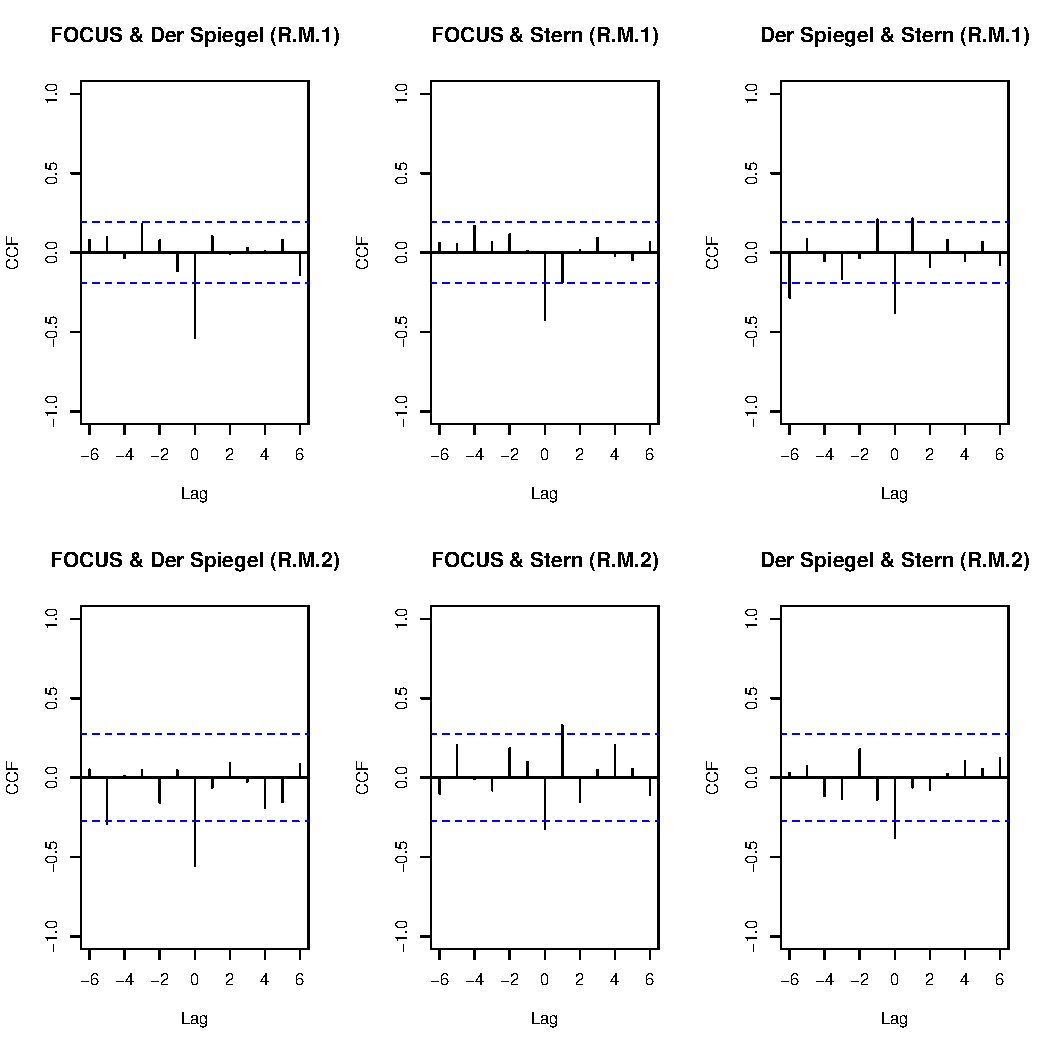
\includegraphics[width=.8\linewidth]{ccf_ads_fss.eps}
	\label{fig_ccf_ads_fss}
\end{figure}



\subsubsection{Comparison with Benchmark}

Figure \ref{fig_QQ_fss} can now be used to compare the results form our empirical analysis with the simulated benchmark. Assuming that total INE (from reader market to advertising market and reverse) exist and are positive, the following conclusions can be drawn: In the reader market, contemporary correlation coefficients ($\rho \in (0.2;0.3)$) suggest, that FOCUS / Der Spiegel most closely resemble each other ($\theta\approx0.2-0.3$). In the later sample the substitutional relationship between Der Spiegel and Stern intensified ($\theta\approx0.3-0.4$).\footnote{Note, that the upper two lines represent the contemporary correlation between sales of FOCUS / Der Spiegel in the reader market for the earlier sample and the lower lines show the estimated cross correlation on the advertising market: The higher the assumed sum of INE, the lower is the indicated $\theta$. To put it differently, the same negative correlation coefficients indicate less competition if the INE is high. For instance, if we assume, that the sum of INE ranges between 0.1 and 0.4, we can find a degree of homogeneity of $\theta=0.6$ on the advertising market, whereas INE of 0.7 to 0.9, indicate $\theta=0.4$. In the later sample, negative correlation between FOCUS / Der Spiegel decreased ($\rho=-0.35$), suggesting a degree of homogeneity of $\theta\approx0.3$ (or $\theta\approx0.2$ if we assume $d+g>0.8$).} 
However, in the advertising market, substitutional relationship between FOCUS and Der Spiegel is stronger than it is in the reader market. Correlation coefficients ranging between $\rho=0.5$ and $\rho=0.6$ indicates that the degree of product differentiation ranges between $\theta=0.4$ and $\theta=0.7$ for the period from 2004 to 2006. 


%\begin{figure}[H]
%	\centering
%	\caption{Degree of competition FOCUS $\&$ Der Spiegel 2004-2006}
%	\label{fig_QQ_fss}
%	\begin{adjustbox}{width=\textwidth}	
%	\input{QQ_fss.tex}
%\end{adjustbox}
%\end{figure}
  
 

Our empirical results imply much stronger substitutional relationships in the advertising market for all pairs of magazines. This strongly supports the assumption of the dichotomy of the two market sides with respect to a market definition. Furthermore, the contemporary correlation in the advertising market decreased between the two periods for FOCUS and Der Spiegel, and slightly increased for FOCUS/Stern and Der Spiegel/Stern. However, the degree of competition between the last two pairs can be assumed to have remained the same. Still, the overall competition in the advertising market seems to have diminished, possibly caused by new, digital advertising possibilities constituting new substitutes for advertising demand. 

Turning to the reader market contemporary substitutional relationship also decreased between the periods regarding FOCUS / Der Spiegel, whereas Der Spiegel / Stern seem to became stronger substitutes. This might be due to a change in the editorial concept of one or both magazines. FOCUS and Stern did not show any significant substitutional relationship in both samples.  

Overall, the empirical results support the assumption, that the three magazines are rather substitutes in the advertising market, but seem to claim own sub-markets in the reader market within both periods. However, during the latter period new products such as online advertising probably reduced the degree of competition in the advertising market. 






\subsection{Program Guides}

A similar analysis as for the news magazines has been conducted for the market of program guides, including the magazines TV-Movie, TV-Spielfilm and TV-Digital. 
Again, unit root tests as well as time pre-whitening have been carried out as a first step. Figure \ref{fig_arima_circ_tv} includes adjusted time series for all TV magazines from both markets.  


Figure \ref{fig_ccf_tv} shows the cross-correlation functions of the reader (R.M.) and the advertising market (A.M.). The magnitude of the contemporary correlation among TV-Movie and TV-Spielfilm is the strongest on both market sides (with $\rho=-.33$ in the reader and $\rho=-.64$ in the advertising market, respectively). Comparing these results with our benchmark model, and assuming positive INE, the competition parameter ranges between $\theta=.3-.5$ in the reader market and $\theta=.4-.6$ in the advertising market. Again, the degree of competition depends on the sum of the indirect network effects: the higher the assumed INE, the lower the competition parameter for the same correlation coefficient. Contemporary correlations between TV-Movie and TV-Digital are statistically significant but rather small in the reader market $\rho=-.20$, indicating degrees of substitutability of $\theta\approx.3$. On the advertising market contemporary correlation is stronger ($\rho = -.42$) indicating a stronger competition in this market side ($\theta\approx.4$). No significant correlation can be found between TV-Spielfilm and TV-Digital.




\begin{figure}[H]
\caption{program guides (adjusted)}
\label{fig_arima_circ_tv}
\begin{minipage}
	\centering
	\input{arima_circ_tv.tex}
\end{minipage}
\hfil
\begin{minipage}
	\centering
	\input{arima_ads_tv.tex}
\end{minipage}
\end{figure}

\begin{figure}[H]
\caption{CCF program guides}
\label{fig_ccf_tv}
	\centering
	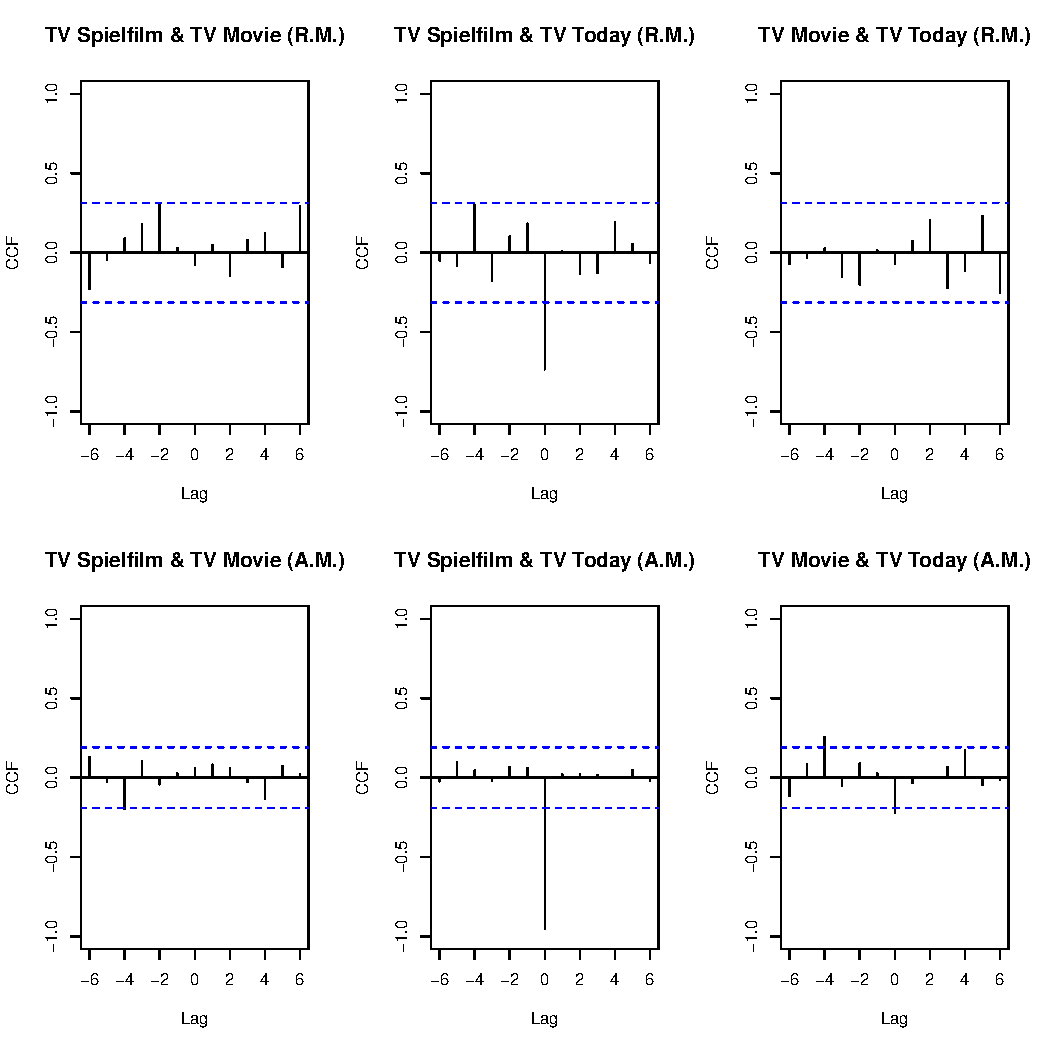
\includegraphics[width=.9\textwidth]{ccf_tv.eps}
\end{figure}




\subsection{Women's Magazines}

The ccf of the adjusted time series are shown in figure \ref{fig_ccf_frauen}. As a striking outcome, contemporary correlation in the reader market is rather small for all three cases, with a value of $\rho=-.29$ Freundin / Für Sie, suggesting a degree of homogeneity of $\theta=.2-.3$. However, on the advertising market contemporary correlation between Brigitte and Freundin is relative large ($\rho=-.57$), whereas contemporal correlation of Brigitte / Für Sie ($-.28$) is smaller, but still significant. No significant correlation can be found between Freundin / Für Sie. The high correlation of Brigitte and Freundin indicates a degree of competition of $\theta=.4-.5$, and $\theta=.2-.3$ for Brigitte / Für Sie. 

Put differently, women's magazines seem to be substitutes only in the advertising but not in the reader market. Although this may seem counter-intuitive, this result is typical for some media markets. As described above, even if different groups of readers do not consider some specific media outlets as substitutes, this does not necessarily imply that advertising customers do not consider the readerships of the magazines as substitutional. 


\begin{figure}[H]
\caption{women's magazines (adjusted)}
\begin{minipage}
	\centering
	\input{arima_circ_frauen.tex}
\end{minipage}
\hfil
\begin{minipage}
	\centering
	\input{arima_ads_frauen.tex}
\end{minipage}
\end{figure}


\begin{figure}[H]
\caption{CCF women's magazines}
\label{fig_ccf_frauen}
	\centering
	\includegraphics[width=.9\textwidth]{ccf_frauen.eps}
\end{figure}


\subsection{Program guides and women's magazines }

In order to test the validity of our method we finally calculated cross correlation functions between women's magazines and TV guides (see figure \ref{ccf_tvfrauen}). As expected, there is no evidence for any significant substitutional relationship. Neither for the reader nor for the advertising market are any statistically significant correlations to be found. This is of course not surprising at all, as TV guides and women's magazines cannot be considered substitutes in the reader market. Similar applies to the advertising market. Although there might be some products for which advertising customers consider TV guides as well as women's magazines as a possible advertising outlets, the readerships of both types of magazines are supposed to be quite different with respect to socio-demographic characteristics. However, socio-demographics is most important for identifying advertising customers' target groups. 

\begin{figure}[H]
\caption{CCF women's magazines and program guides}
\label{ccf_tvfrauen}
	\centering
	\includegraphics[width=.9\textwidth]{ccf_tvfrauen.eps}
\end{figure}




\section{Conclusions}

Market definition in two-sided markets is a complex challenge and until now no method has been developed which is applicable and suitable as a practical  antitrust tool. Usual methods developed for on-sided markets are no longer valid and the interdependence of quantities and prices from both markets, caused by indirect network effects, leads to severe identification problems. For this reason, some authors recommend to completely abandon market definition as it is considered useless and incoherent (Kaplow, 2010; Evans...). However, competition authorities are either obliged to define markets or have at least to identify the closest competitors in order to evaluate effects of possibly anti-competitive behaviour.   

For this reason, we developed a new method for the identification of competitors in two-sided markets by using time series methods and simple correlation analysis. At first, time series on quantities from both markets are adjusted by time series models in order to prevent spurious regressions. We use quantities instead of prices as (i) substitutability is directly reflected in quantities but not necessarily in prices (ii) indirect network effects are directly linked to quanitites  and (iii) two-sided markets such as platform markets typically characterized by zero prices on either of the sub markets. Next, either cross-correlation functions or simple contemporary correlations are calculated to identify the substitutability of different products. The procedure is applied to reader and advertising markets of different popular magazines genres. 

To evaluate the degree of substitutability between different media outlets, we first build a simple model of two-sided markets. We then use Monte Carlo simulations in order to calculate correlation coefficients for varying degrees of product differentiation as well as indirect network effects. A comparison of empirical correlations with Monte Carlo results can then be used to identify the degree of substitutability. 

The conclusions from our empirical analysis is twofold: First, our method seems to be appropriate to estimate degrees of substitutability in two-sided markets. The results seem to be reasonable and valid. Correlation coefficients are surprisingly different between seemingly similar products. This applies especially to circulation. 

Second, our analysis shows that market definition is likely to be asymmetric between different markets (i.e., the reader and the advertising market). While circulation between most products shows only a moderate substitutability, correlations in advertising market seem to be much higher. These results are also in ine with our theoretical considerations. 

As we have so far analysed only a small number of magazines, the next step in our analysis is to include a much higher number of outlets from different segments. Especially online platforms markets are an interesting research objects, as many recent antitrust cases affect digital platforms. 


% ----------------------------------------------------------------------------------------------------
%  APPENDICES
% ----------------------------------------------------------------------------------------------------

\printbibliography

\begin{appendices}



% MODEL

%\chapter{Model}

%\subsection{Profit Maximization}\label{appendix_model}






% EMPIRCAL ANALYSIS

\section{Empirical Analysis}

\subsection{Autocorrelation function (ACF) of adjusted time series}

\subsubsection{News Magazines}\label{app_acf_fss}

\begin{figure}[H]
\caption{news magazines: reader Market}
	\centering
	\includegraphics[width=.9\linewidth]{resid_acf_circ_fss.eps}
\end{figure}

\begin{figure}[H]
\caption{news magazines: advertising market}
	\centering
	\includegraphics[width=.9\linewidth]{resid_acf_ads_fss.eps}
\end{figure}

(1) = 2004w33-2006w33, (2) = 2013w33-2015w33

\subsubsection{Program Guides}\label{appendix_sum_tv}

\begin{figure}[H]
\begin{minipage}{.5\textwidth}
	\centering
	\captionof{figure}{reader market}
	\includegraphics[width=.9\textwidth]{resid_acf_circ_tv.eps}
\end{minipage}
\hfil
\begin{minipage}{.5\textwidth}
	\centering
	\caption{advertising market}
	\includegraphics[width=.9\textwidth]{resid_acf_ads_tv.eps}
\end{minipage}
\label{resid_acf_tv}
\end{figure}

\subsubsection{Women's Magazines}

\begin{figure}[H]
\begin{minipage}{.5\textwidth}
	\centering
	\captionof{figure}{reader market}
	\includegraphics[width=.9\textwidth]{resid_acf_circ_frauen.eps}
\end{minipage}
\hfil
\begin{minipage}{.5\textwidth}
	\centering
	\caption{advertising market}
	\includegraphics[width=.9\textwidth]{resid_acf_ads_frauen.eps}
\end{minipage}
\label{resid_acf_frauen}
\end{figure}


\subsection{Philipps & Perron test for Unit Root}

%%%%%%%%%%%%% Without Trend %%%%%%%%%%%%%%%

\begin{table}[!htbp]\centering 
  \caption{Unit Root Test, no trend} 
  \label{tab_uroot} 
\begin{tabular}{@{\extracolsep{5pt}} llll} 
\\[-1.8ex]\hline 
\hline \\[-1.8ex] 
 & FOCUS & Der Spiegel & Stern \\ 
\\[-1.8ex]\hline 
\hline \\[-1.8ex] 
2004 - 2006 \\
\hline
Sales & -8.20 & -5.27 & -6.01 \\ 
Ad pages & -3.49 & -3.33 & -3.60 \\ 
\hline
2013 - 2015 \\
\hline
Sales & -10.69 & -7.63 & -8.51 \\ 
Ad pages & -3.83 & -4.50 & -4.99 \\ 
\hline
Sig. Level & 1pct & 5pct & 10pct \\ 
Critical Values & -3.49 & -2.89 & -2.58 \\ 
%%%%%%% Program Guides 
\\[-1.8ex]\hline 
\hline \\[-1.8ex] 
 & TVMovie & TVSpielfilm & TVDigital \\ 
\\[-1.8ex]\hline 
\hline \\[-1.8ex] 
Sales & -0.02 & -0.15 & -1.66 \\ 
Ad pages & -4.14 & -4.34 & -5.74 \\
\hline 
Sig. Level & 1pct & 5pct & 10pct \\ 
Critical Values & -3.52 & -2.90 & -2.9 \\ 
%%%%%%% Womens Magazines  
\\[-1.8ex]\hline 
\hline \\[-1.8ex] 
 & Brigitte & Freundin & Für Sie \\ 
\\[-1.8ex]\hline 
\hline \\[-1.8ex] 
Sales & -5.96 & -7.87 & -4.66 \\ 
Ad pages & -4.87 & -4.15 & -5.26 \\ 
\hline
Sig. Level & 1pct & 5pct & 10pct \\ 
Critical Values & -3.52 & -2.90 & -2.59 \\ 
\hline \\[-1.8ex] 
\end{tabular} 
\end{table} 

\end{appendices}


\end{document}
